\documentclass{beamer}

\usetheme{Madrid}
\usecolortheme{crane}

\title{A LaTeX Használatának Előnyei}
\author{Gecse Tamás}
\date{\today}

\usepackage{graphicx}
\usepackage{listings}
\usepackage{tikz}
\usepackage{hyperref}
\usepackage{amsmath}
\usepackage[version=4]{mhchem}
\usepackage{chemfig}
\usepackage{multicol}
\usepackage{chessboard}
\usepackage{media9}  % Csomag a videók beágyazásához

\begin{document}

\begin{frame}
    \titlepage
\end{frame}

\begin{frame}
    \tableofcontents
\end{frame}

\section{Bevezetés}
\begin{frame}
    \frametitle{Bevezetés}
    A LaTeX egy erőteljes szövegszerkesztő, amely különösen népszerű tudományos dokumentumok írására.
\end{frame}

\section{Főbb Előnyök}
\begin{frame}
    \frametitle{Főbb Előnyök}
    \begin{itemize}
        \item Professzionális megjelenés
        \item Könnyű matematikai formulák kezelése
        \item Rugalmas struktúrák kialakítása
        \item Széleskörű testreszabási lehetőségek
    \end{itemize}
\end{frame}

\section{Képek és Grafikák}
\begin{frame}
    \frametitle{Képek és Grafikák}
    \begin{figure}
        \centering
        
\includegraphics[width=0.6\textwidth]{neko.jpg}
        \caption{Példa kép}
    \end{figure}
\end{frame}

\section{Programkód}
\begin{frame}[fragile]
    \frametitle{Programkód Példa}
    \begin{lstlisting}[language=C++, caption=Hello World C++ Program]
    #include <iostream>
    using namespace std;

    int main() {
        cout << "Hello, World!" << endl;
        return 0;
    }
    \end{lstlisting}
\end{frame}

\section{Matematikai Formulák}
\begin{frame}
    \frametitle{Matematikai Formulák}
    Az alábbi formula az integrál definícióját mutatja be:
    \begin{equation}
        \int_{a}^{b} f(x) \, dx = F(b) - F(a)
    \end{equation}
\end{frame}

\section{Kémiai Képletek és Ábrák}
\begin{frame}
    \frametitle{Kémiai Képletek}
    \begin{itemize}
        \item A víz kémiai képlete: \ce{H2O}
        \item Az etanol kémiai képlete: \ce{C2H5OH}
        \item A glükóz kémiai képlete: \ce{C6H12O6}
    \end{itemize}
\end{frame}

\begin{frame}
    \frametitle{Kémiai Szerkezetek}
    A glükóz szerkezeti ábrája:
    \begin{center}
        \chemfig{*6((-OH)-[::-1](-O)-[::-1](-OH)-[::-1](-H)-[::-1](-H)-[::-1](=O))}
    \end{center}
\end{frame}

\section{Sakkállás Példa}
\begin{frame}
    \frametitle{Sakkállás Példa}
    Az alábbi táblán egy legális állás látható, ahol a fehér játékos következik:
    \begin{center}
        \chessboard[
            setpieces={
                Ke1, Qd1, Bb5, Nc3, Pd4, Pg2, Pf2, % fehérek
                pg7, ph7, kb8, qc7, bb7, ra8, pe4 % feketék
            }
        ]
    \end{center}
\end{frame}

\section{Videó Példa}
\begin{frame}
    \frametitle{Videó Példa}
    \centering
    \includemedia[
        activate=onclick,
        width=10cm,
        height=7cm,
        3Dtoolbar, 
        transparent,
    ]{ 
\includegraphics{cat.png}}{cat.mp4} % A videó fájl neve
\end{frame}

\section{Kereszthivatkozások}
\begin{frame}
    \frametitle{Kereszthivatkozások}
    A LaTeX lehetőséget biztosít kereszthivatkozások létrehozására:
    \begin{itemize}
        \item \hyperlink{sec:introduction}{Bevezetés}
        \item \hyperlink{sec:benefits}{Főbb Előnyök}
    \end{itemize}
\end{frame}

\section{TikZ Grafika}
\begin{frame}
    \centering
    \frametitle{TikZ Grafika}
    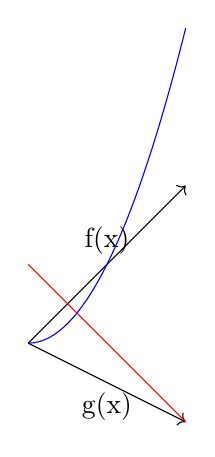
\begin{tikzpicture}
        \draw[->] (0,0) -- (2,2) node[midway, above] {f(x)};
        \draw[->] (0,0) -- (2,-1) node[midway, below] {g(x)};
        \draw[domain=0:2,smooth,variable=\x,blue] plot ({\x},{\x*\x});
        \draw[domain=0:2,smooth,variable=\x,red] plot ({\x},{-\x+1});
    \end{tikzpicture}
\end{frame}

\section{Irodalomjegyzék}
\begin{frame}
    \frametitle{Irodalomjegyzék}
    \begin{thebibliography}{9}
        \bibitem{lamport}
            Leslie Lamport,
            \textit{LaTeX: A Document Preparation System},
            Addison Wesley, 1986.
        \bibitem{knuth}
            Donald E. Knuth,
            \textit{The TeXbook},
            Addison Wesley, 1984.
    \end{thebibliography}
\end{frame}

\begin{frame}
    \frametitle{Összefoglalás}
    \begin{itemize}
        \item A LaTeX egy hatékony eszköz tudományos írásra.
        \item Széleskörű testreszabási lehetőségeket kínál.
        \item Számos funkcióval segíti a felhasználókat.
    \end{itemize}
\end{frame}

\end{document}
